\documentclass[platex,dvipdfmx,a4paper,twocolumn,base=10pt,jbase=10pt,ja=standard]{bxjsarticle}
% \documentclass[uplatex,dvipdfmx,a4paper,twocolumn,base=11pt,jbase=11pt,ja=standard]{bxjsarticle}
% https://github.com/yk-lab/ipsj_national_convention_template

\usepackage{ipsj}

\usepackage[dvipdfmx]{graphicx}
\usepackage{amsmath,amsfonts}
\usepackage{bm}

% \def\baselinestretch{1.0}
\def\baselinestretch{0.9}  % 0.86

\title{\Large\bf 電子教材の閲覧データとコンテンツ内容を用いた\\学習者のスコア予測}{\bf Predicting learner scores using browsing data and content of electronic learning materials}
\author{兵庫県立大学 社会情報科学部}{小岸 沙也加}{Sayaka Kogishi, University of Hyogo}
\author{九州大学 データ駆動イノベーション推進本部}{峰松 翼}{Tsubasa Minematsu, Kyushu University}
\author{九州大学 大学院システム情報科学研究院}{島田 敬士}{Atsushi Shimada, Kyushu University}
\author{兵庫県立大学 大学院情報科学研究科}{川嶋 宏彰}{Hiroaki Kawashima, University of Hyogo}

\begin{document}
\maketitle

\section{はじめに}
\label{sec:intro}
    
%近年,学校の講義では講義
%小学生から大学生まで
初等中等教育から高等教育まで,タブレットやノートPCが幅広く普及し,講義資料の閲覧や課題の提出等で用いられるようになっている.講義資料の閲覧や操作では,オンラインで配布されたPDF等の資料をダウンロードしてオフラインで閲覧する形態だけではなく,デジタル教材の配信システム上に教師がアップロードした講義資料をオンラインで閲覧する形態もある.後者の形態では,いつどの学生が
%どのコンテンツの
% どのページでどのような操作をしたかという,詳細な閲覧データ(操作ログ)を取得できる.
% この閲覧データを解析することで各学生の理解度やつまずき箇所を推定できれば,個々の学生に早い段階でアプローチすることができ,学生の学力向上に繋がると期待できる.
どのページでどのような操作をしたかという,詳細な操作ログを取得できる.
この閲覧データを解析することで各学生の理解度や,つまずき箇所を推定できれば,個々の学生に早い段階でアプローチすることができ,学生の学力向上に繋がると期待できる.

%そこで本研究では,デジタル教材の配信システムのひとつである,BookRollシステムから得た閲覧データを用いて学生の学習行動から各学生に対し教材の理解度推定を行う.学生の学習行動から理解度推定ができれば,小テストや定期テストの前の早い段階で各個人に適したアプローチすることができるようになり,学生の学力向上に繋がると期待できる.

% 本研究では理解度を小テストの点数として,閲覧データだけでなく,実際に講義で用いられたコンテンツ内容を使用し毎週講義後に行われる小テストの点数予測を行う.学生の行動に焦点をあて,点数予測を行っている例は以前にもあるため,コンテンツ内容を含めることでどこまで精度があがるのかという点を本研究のリサーチクエスチョンにあげる.

学生の行動から成績予測を行った研究として,デジタル教材の配信システムのひとつである BookRoll システムから得た閲覧データを用いて,毎週の生徒の成績を予測し,
受講期間中に随時リスクのある学生とない学生に分類する試み~\cite{Predictionstudentperformance2022}や,
%講義が終わる前にリスクのある生徒とない生徒に分類する試み~\cite{Predictionstudentperformance2022}や,
%LRP (Layer-wise Relevance Propagation) と呼ばれる
ニューラルネットワークの解釈手法を用いて
%最終成績の上位,中位,下位に分類する研究
どのような学習行動が成績に関連するかを調べた研究~\cite{BR12020}がある.一方で,閲覧コンテンツそのものの情報も成績予測には有効である可能性があるが十分検証されていない.
%を積極的に利用する
%ことで,予測精度
%が向上する可能性については十分検証されていない.
%また,BookRollシステムから得たデータを使用した研究として,
%ではLRPというを行っている.

%学生の行動から成績予測を行った研究として,
%~\cite{Predictionstudentperformance2022}ではBookRollシステムで取得した講義資料の読書行動から毎週の生徒の成績を予測し,講義が終わる前にリスクのある生徒とリスクのない生徒に分類することが可能と発表している.

%BookRollシステムから得たデータを使用した研究として,~\cite{BR12020}ではLRPというニューラルネットワークの解釈手法を用いて最終成績の上位,中位,下位の分類を行っている.

そこで本研究では,学習者の行動を記録した閲覧データに加えて,講義で使用されたスライドなどの講義資料(本稿では「コンテンツ」と呼ぶ)のテキスト情報を利用することで,各学生の理解度の推定精度向上を目指す.
ここで理解度とは,毎週講義後に行われる小テストの点数(スコア)とし,閲覧データはBookRollシステムで得られた操作ログを用いる.このとき,コンテンツ情報の利用が小テストのスコア予測にどれだけ貢献するかを検証する.
%を通じて,利用することで予測精度がどのように向上するかを明らかにする.

% 理解度を小テストの点数(スコア)として,毎週講義後に行われる小テストのスコア予測を行う.予測には閲覧データだけではなく,実際に講義で用いられたコンテンツの内容を使用する.学生の閲覧行動のみを用いる場合と,コンテンツ内容を含めた場合とで,予測精度がどのように変化するかを評価する.本研究のRQはコンテンツ内容を含めることでどこまで精度があがるのかである.



%\section{関連研究}
%\label{sec:Related}




%\section{BookRollシステム}
%\label{sec:BookRoll}

\noindent{\bf BookRollシステム}\quad 
BookRollシステム~\cite{BookRoll}は,教員がアップロードした講義資料や教材を学生がオンライン上で閲覧できるシステムである.
%図1にBookRollシステムの操作画面の一例を示す.
%BookRollシステムでは
%各ページに対しブックマーク,メモの記入,マーカーをつける,コンテンツ内を検索するなどの機能がある.
% \vspace{-10mm}
% 
% \begin{figure}[h]
%   \centering
%   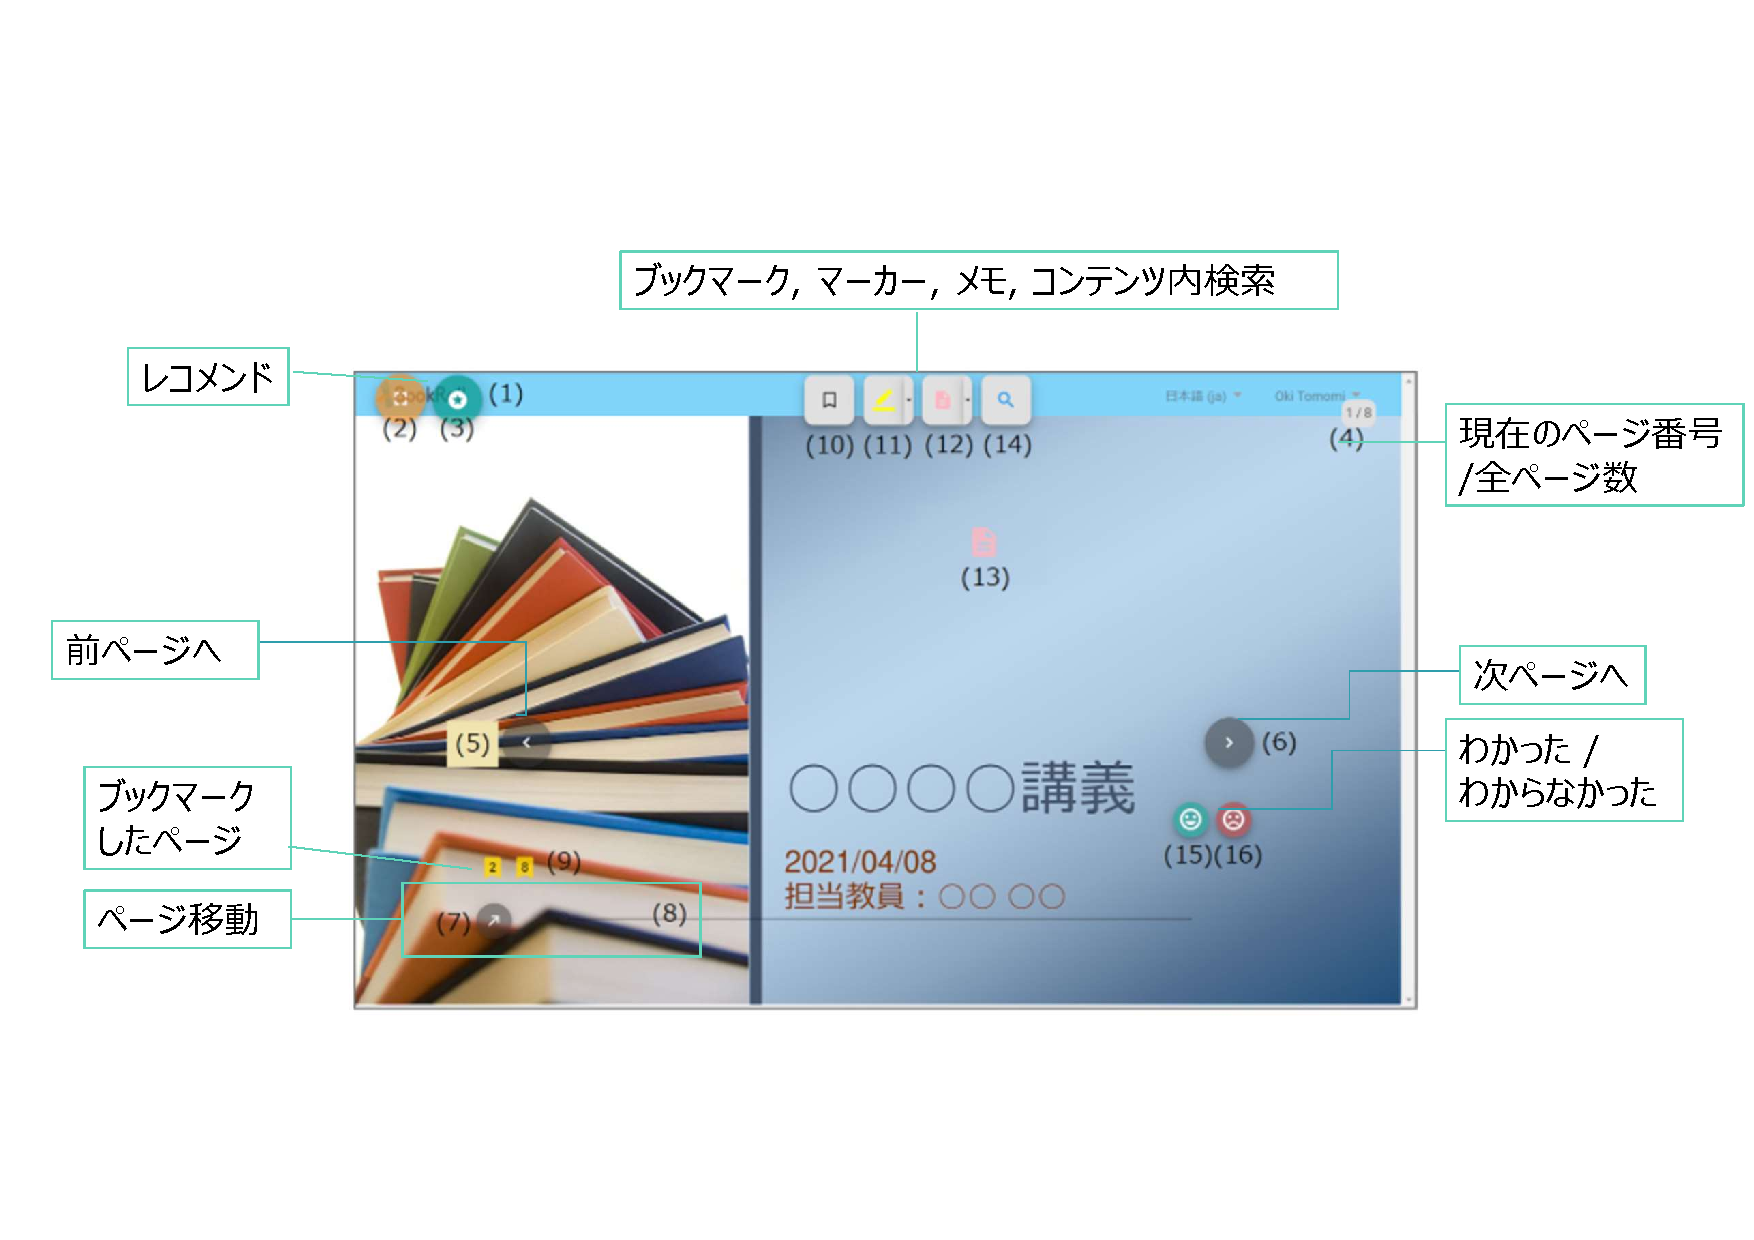
\includegraphics[scale = 0.3]{BookRoll.pdf}
%   \vspace{-15mm}
%   \caption{BookRollシステム操作画面例}
%   \label{fig:BookRollシステム操作画面例}
%  \end{figure}
%
% 閲覧データはコンテンツを開く,閉じる,次のページへ進む,一つ前のページへ戻るなどの行動がされたタイミングで操作を行った学生のID,行動をした日時,コンテンツ番号,ページ番号,どのような操作を行ったか等の情報が記録される.記録される主な内容を表1に示す.表1のoperation\_nameにあたる,閲覧データに記録される操作の一部を表2に示す.
%
閲覧データとしては,たとえばコンテンツを開く/閉じる,次のページへ進む,一つ前のページへ戻る,マーカーやメモを付与する,コンテンツ内検索を行うといった操作を行ったタイミングで,その操作タイプが,操作を行った学生のID,日時,コンテンツ番号,ページ番号,操作タイプなどの情報と共に記録される.
%記録される操作には,ページ移動,マーカー,メモ,ブックマークをつける/消す,コンテンツ内検索を行うなどが含まれる.

% \begin{table}[h]
%   \centering
%   \begin{tabular}{c|l}
%     記録名 & 内容 \\ \hline
%     contents\_id/name & コンテンツID/名 \\ 
%     marker\_position/color & マーカーをつけた場所/色 \\ 
%     memo\_text & メモの内容 \\
%     operation\_date & 操作した日時 \\ 
%     operation\_name & 操作内容 \\ 
%     page\_no & 操作したページ番号 \\ 
%     userid & 学生に割り振られた番号 \\ \hline
%   \end{tabular}
%   \caption{記録される主な内容}
%   \label{tb:記録される主な内容}
% \end{table}

% \begin{table*}[h]
%   \centering
%   \begin{tabular}{c|l}
%     operation\_name & 内容 \\ \hline
%     OPEN & コンテンツを開く \\ 
%     CLOSE & コンテンツを閉じる \\ 
%     NEXT & 次のページへ移動 \\
%     PREV & ひとつ前のページへ移動 \\ 
%     PAGE\_JUMP & 特定のページへ移動 \\ 
%     ADD/DELETE BOOKMARK & ブックマークをつける/消す \\
%     ADD/DELETE MERKER & マーカーをつける/消す \\
%     ADD/DELETE MEMO & メモをつける/消す \\
%     SERCH & コンテンツ内検索を行う \\
%     GETIT & わかったボタンを押す \\ 
%     NOTGETIT & わからなかったボタンを押す \\
%     OPEN\_RECOMMENDATION & 関連サイトを開く \\ \hline
%   \end{tabular}
%   \caption{操作内容の一部}
%   \label{tb:操作内容の一部}
% \end{table*}

% \section{データ関連の情報・分析結果}



% \noindent{\bf オーブンの温度}\quad
% Subsection がスペース的にきつい場合は,パラグラフにする手もある(国際会議ではよく使われる).本文テスト本文テスト本文テスト本文テスト本文テスト本文テスト本文テスト本文テスト本文テスト本文テスト

% \noindent{\bf Let's bake.}
% 英語の論文だとパラグラフタイトルの後にピリオドを入れる.本文テスト本文テスト本文テスト本文テスト本文テスト本文テスト本文テスト本文テスト本文テスト本文テスト


\section{コンテンツを利用したスコア予測}
\label{sec:scoreprediction}

% 全体像入れる?
% 漢数字とアラビア数字ぐっちゃぐちゃ

% 定義の話もする?
% スライドは講義資料の1ページ単位のこと->ページ?
% コンテンツは週に使われるスライド全体のこと
% 次元かく

図~\ref{fig:overview}は本研究の全体像である.
%行動がされる度に取得できる閲覧データから
BookRollから得られた閲覧データより,各学生について,あるコンテンツの各ページにおける操作タイプごとの操作回数および閲覧時間を求め,これら特徴量を要素とするようなベクトルを各学生の「行動特徴ベクトル」と呼ぶ.
% ここからはまだ (2022.12.16)
%行動特徴ベクトルはコンテンツごとに求めるものとする.
ここで,学生$i$のコンテンツ$c$における行動特徴ベクトルを$\bm{u}^{(i)}_c$と表す.
$\bm{u}^{(i)}_c$の次元数は「ページ数 $\times$ (操作タイプ数 + 1)」(最後の1は閲覧時間に対応)であり,ページ数はコンテンツ$c$によりそれぞれ異なる.
% ページ数×行動数?
% 使用する行動を絞っていることは

\begin{figure}[tbp]
  \centering
  %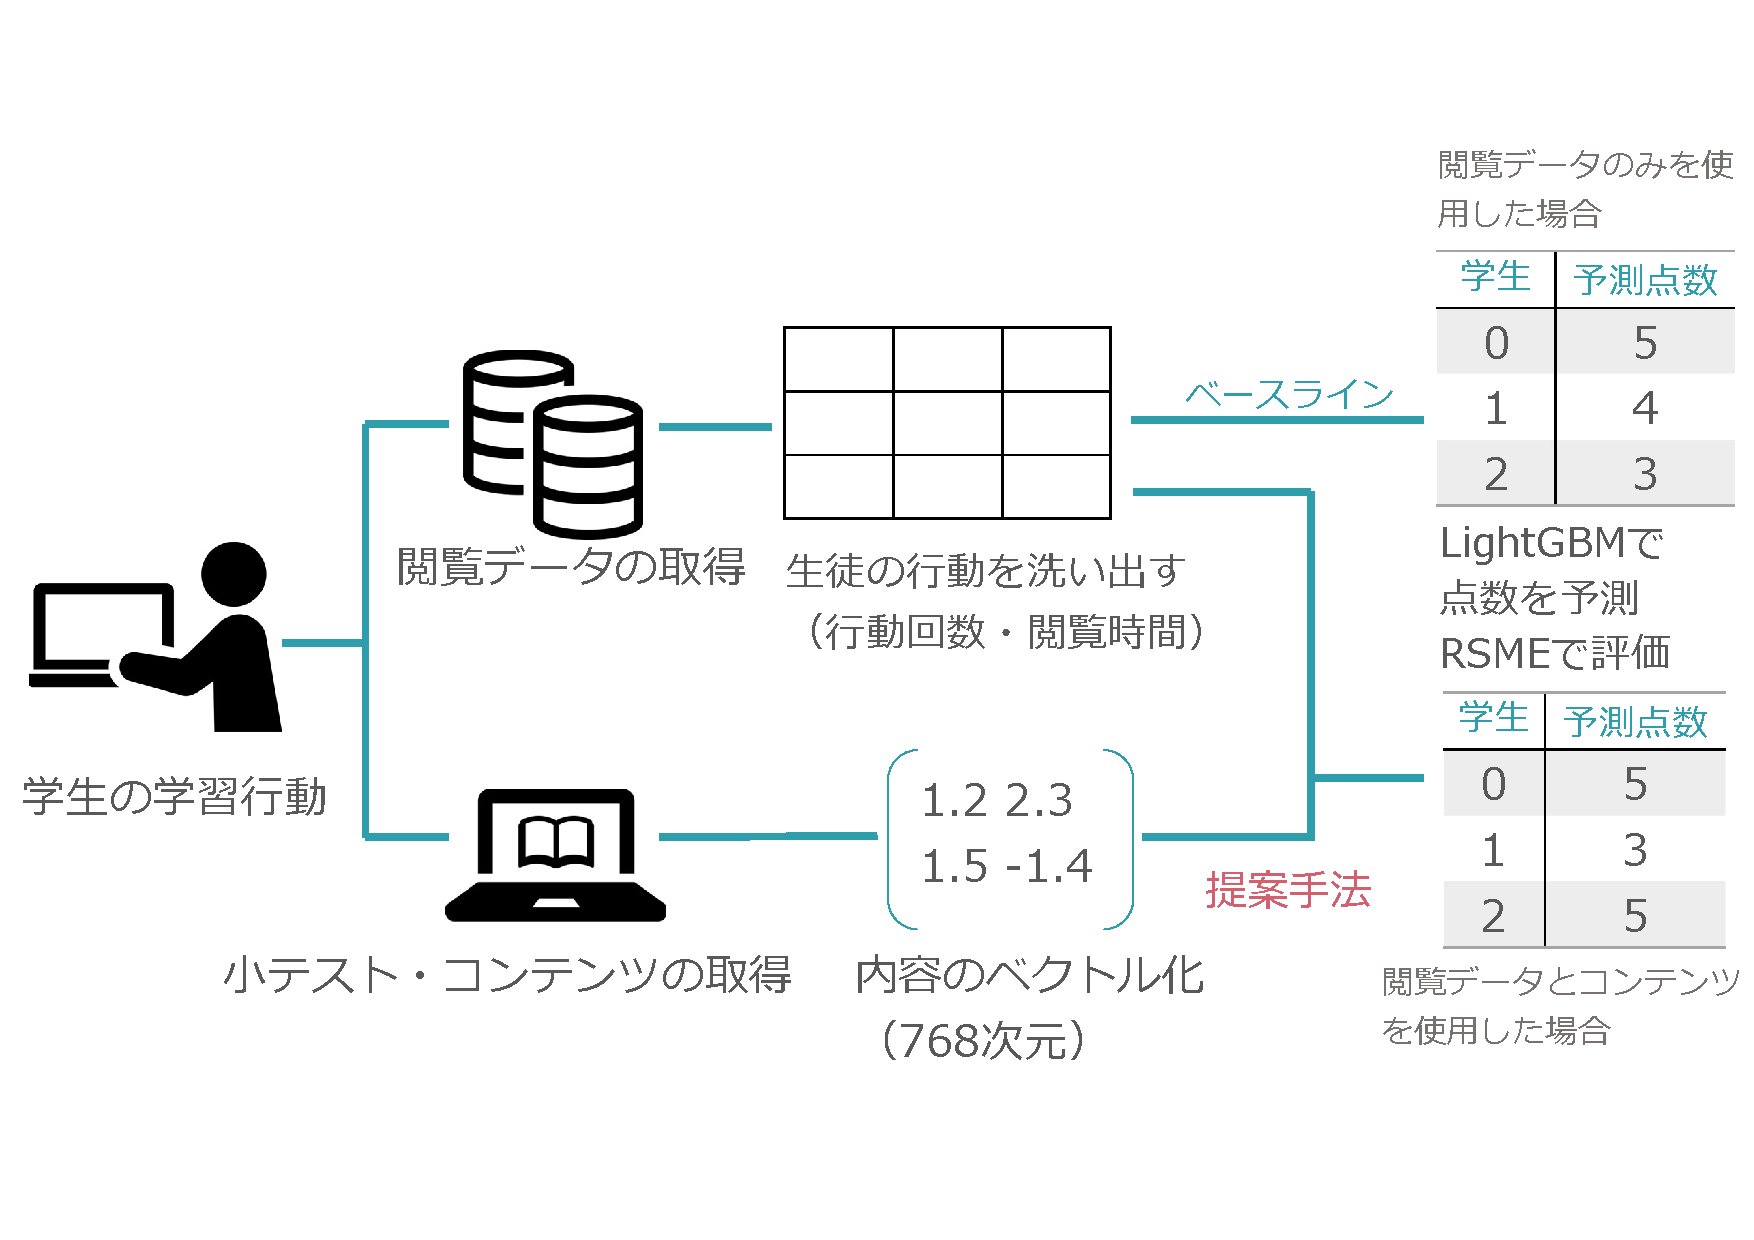
\includegraphics[scale = 0.23]{zentaizo.pdf}
  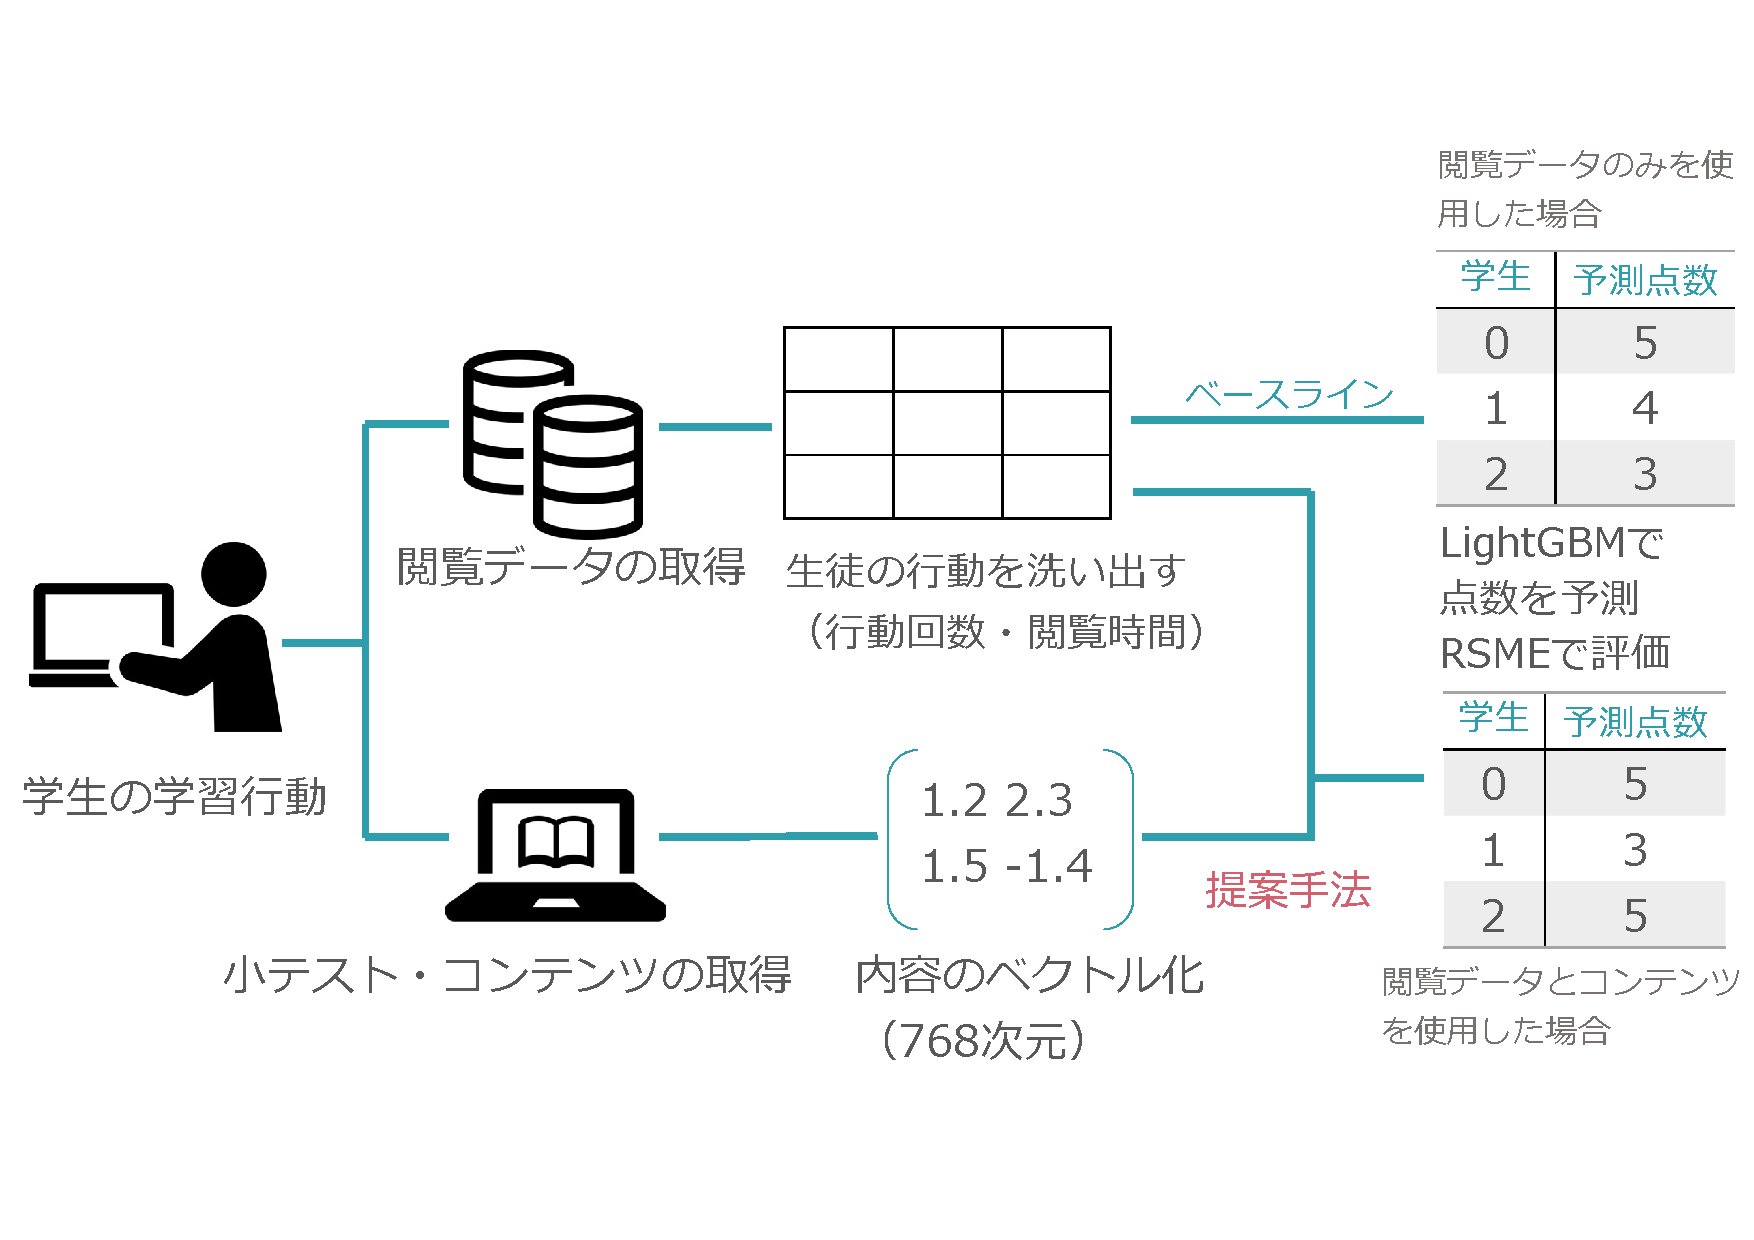
\includegraphics[width=0.9\linewidth]{zentaizo.pdf}
  \vspace{-8mm}
  \caption{本研究の全体像}
  \label{fig:overview}
  \vspace{-8mm}
\end{figure}

%一列のベクトルを求める.これを学生の行動特徴量と呼ぶ.
%本研究ではこのベクトルで表現される行動特徴量にコンテンツ内容を加えて点数予測を行う方法を提案する.
本研究では,さらに学生$i$がコンテンツ$c$においてよく閲覧したページの内容情報を多く含む「閲覧コンテンツベクトル」$\bm{v}^{(i)}_c$を求め,行動特徴ベクトルに連結する.この統合された特徴ベクトルを用いて,小テストのスコア予測を行う方法を提案する.
ベースラインとして,行動特徴ベクトルのみを使用した場合でもスコア予測を行い,予測精度を比較する.

% 言い方わからない


% 行動特徴量として行動回数洗い出す操作は,すべての操作ではなく,OPEN, NEXT, PREV, CLOSE, PAGE\_JUMP, GETIT, OPEN\_RECOMMENDATION, CLOSE\_RECOMMENDATION, NOTGETIT, ADD MARKER, DELETE MARKER, CLICK\_RECOMMENDATION, open\_timeに絞る.

\noindent{\bf 閲覧コンテンツベクトル}\quad
まず,コンテンツ${c}$に含まれる各ページのテキスト情報のベクトル化を行う.
%そのベクトルを行動特徴量に付け加えて点数予測を行う方法である.
%現在は
% ベクトル化には,事前学習済みのSentence-BERT~\cite{sentence-BERT2019}を使用するものとし,これによりページ$p$ごとに768次元の「ページベクトル」$\bm{v}_{(c,p)}$が得られる.ただし単位ベクトルに正規化を行った.
ベクトル化には,事前学習済みのSentence-BERT~\cite{sonoisa}を使用するものとし,これによりページ$p$ごとに768次元の「ページベクトル」$\bm{v}_{(c,p)}$が得られる.ただし単位ベクトルに正規化を行った.
%てページ${p^{(c)}}$ごとに768次元のベクトル化を行う.
%しかし,ページ内容をベクトル化したものを付け加えただけでは全ての学生が同じベクトルをもつことになるため,ページベクトルに重みづけを行うことで学生ごとに違ったベクトルを作成する.
ここで,各学生がよく閲覧したページの内容情報を多く含むようなベクトルを得るために,学生$i$のページ$p$に対する閲覧時間の総和$t^{(i)}_{(c,p)}$に基づいてページベクトルに重みづけを行って足し合わせる.具体的には,
%重みには各スライドの閲覧時間$t^{(i)}_{(c,p)}$を使用し,学生の閲覧時間が長いスライドほど重要度$w^{(i)}_{(c,p)}$を高く設定する.
%単純に閲覧時間が長いほど重要度を高くすると異常に長い時間閲覧していると記録されている可能性があるため,一度に同じページを見ている時間が17分(1020秒)以上の場合はセッションタイムアウトによりCLOSEが記録されなかった,もしくは長時間放置されているものとしてフィルタ―をかける.フィルタ―をかけたあとの閲覧時間をページごとに足し合わせた時間を使用し,重要度を求める.
%各講義回ごとに
%まずコンテンツ$c$内で閲覧時間が最も長いページを求め,その閲覧時間を$t^{(c)}_{max}$とする.
%ここから,各ページの重み $w^{(i)}_{(c,p)} = \frac{t^{(i)}_{(c,p)}}{t^{(c)}_{max}}$ を求め,
%この重みを用いて
閲覧時間をそのまま各ページの重み $w^{(i)}_{(c,p)} = t^{(i)}_{(c,p)}$として
ページベクトルの線形和 $\bm{v}^{(i)}_c = \sum_p w^{(i)}_{(c,p)}\bm{v}_{(c,p)}$ を求め,単位ベクトルに正規化して閲覧コンテンツベクトルとする.
ただし,同じページを継続して5分より長く開いていたログは,長時間放置されたものとして,各ページの閲覧時間の総和から除外した.
%そこから連続的に重要度を求める.
% 重要度は以下のように求める.
%\begin{align}
%  w^{(i)}_{(c,p)} = \frac{t^{(i)}_{(c,p)}}{t^{(c)}_{max}}
%\end{align}
%ベクトルは各スライドに対し作成されているため,このままでは行動特徴量が大きくなるので,重みづけを行ったベクトルを足し合わせることでベクトルの圧縮を行う.

% 学生番号を$i$とし,各学生の閲覧時間
% c=[1,1+,2-1,2-2,3,4,5,6,7]
% p=[週によって違う]
% 閲覧時間はさらっと言って大丈夫なんか?ページ移動からだすってかく?必要ある?

% 使用する行動は記録されている全ての行動ではなく,絞っている.(ベクトル圧縮のため)言わないといけない(下でかく?)
% 使っている行動の選定理由は行動だけで週ごと予測をしたときに重要であるとでてきた行動(正確には削ったのが、どの週でも重要度が0ってでてきた行動)

% 講義時間外も含む全てのデータと講義時間内\&前後1時間に絞ったのは自分のやりたいこと、目的的に講義時間内に絞ることは必要なのではと思ったから





\section{評価}
\label{sec:evaluation}

%\subsection{使用データセット}
\subsection{データセット}

%2020年に九州大学で行われた講義で使用されたBookRollシステムから得た閲覧データとコンテンツ情報,毎週講義後に行われる小テストから得たデータを使用する.
2020年に九州大学の情報系科目の講義で取得されたBookRollシステムの閲覧データ,講義で用いられたコンテンツ,および講義中に行われた小テストの結果(小テストデータ)を用いる.

%講義は80分講義,10分小テストという形式で100名の学生に対し7週間にわたって行われ,閲覧データは合計200,818ログ記録されている.
講義は100名の学生に対し90分授業が7週間に渡って行われ,各授業の最後の約10分間で小テストが行われた.閲覧データは計200,818行のログからなる.
%
%小テストは5問の択一式の問題で構成され,小テストデータは
小テストは5問の択一式の問題であり,学生が小テストを提出したタイミングで,問題の文章,学生の選択した選択肢,正解か否か,および提出時間が記録される.
%小テストデータには,問題の文章,学生の選択した選択肢,正解か否か,および提出時間が含まれる.
%含まれている.



\subsection{予測および評価方法}

スコア予測は小テストごとにLightGBMを使用して行う.5-fold交差検証を用いて各foldのRMSEの平均により評価する.
評価には小テストごとに求めた5点満点のスコアを使用する.
2週目は2つのコンテンツが使用され,小テストが2回分行われたため,2週目(1)と2週目(2)に分けてスコア予測を行う.
%評価には小テストデータから得た,小テストごとに求めた5点満点のスコアを使用する.
% 今回は
%行動特徴量を講義時間外の行動もすべて含む行動特徴量を使用してスコア予測を行った結果と,講義時間内と前後1時間の行動に絞った行動特徴量を使用して点数予測を行った結果をそれぞれ評価し,ベースラインの結果と提案手法の結果を比較する.

行動特徴ベクトルは,講義時間外の操作を全て用いる場合 (all) と,講義時間内および前後1時間の操作に絞った場合 (in-lec) の2通りで計算し比較する.
%行動特徴量として行動回数洗い出す操作はすべての操作ではなく,閲覧時間を除く,行動回数のみを使用し週ごとの点数予測をLightGBMで行った結果,どの週でもImportanceが0であった行動を除いたOPEN, NEXT, PREV, CLOSE, PAGE\_JUMP, GETIT, OPEN\_RECOMMENDATION, CLOSE\_RECOMMENDATION, NOTGETIT, ADD MARKER, DELETE MARKER, CLICK\_RECOMMENDATION, open\_timeに絞る.
%に用いる操作タイプとして,重要度の低いものは除外した.具体的には,
行動特徴ベクトルに含める操作タイプは,
%各操作タイプの回数を特徴量として
事前にLightGBMで各小テストのスコア予測を行った際に,いずれの小テストでも予測結果への寄与度が0であった操作タイプを除いた.
%具体的には OPEN, NEXT, PREV, CLOSE, PAGE\_JUMP, GETIT, OPEN\_RECOMMENDATION, CLOSE\_RECOMMENDATION, NOTGETIT, ADD MARKER, DELETE MARKER, CLICK\_RECOMMENDATION, open\_time を用いた.

%次元数はコンテンツごとに異なり,1週目1,042次元,2週目(1)1,627次元,2週目(2)1,575次元,3週目1,159次元,4週目1,406次元,5週目1,146次元,6週目1,367次元,7週目1,835次元である.

% p*(12+1)+$\bm{v}^{(i)}_c$次元

% 次元数どうやってかく?表?言葉?表にするとまた伸びる


% Importanceが0であったかどうかはわからないけど先生たちに必要ないって言われた行動も消しています.
% 使用operation
% ['OPEN', 'NEXT', 'PREV', 'CLOSE', 'PAGE_JUMP', 'GETIT', 'OPEN_RECOMMENDATION', 'CLOSE_RECOMMENDATION', 'NOTGETIT', 'ADD MARKER', 'DELETE MARKER', 'CLICK_RECOMMENDATION', 'open_time']

% 削るoperation
% ['TIMER_STOP', 'TIMER_PAUSE', 'MEMO_TEXT_CHANGE_HISTORY']
% 理由:TIMERに関しては無視していいって言われた
% MEMO~の方は学生がメモしている最中が全部記録されるので打ち間違いとかも入る(いらない)

% ['ADD MEMO', 'ADD BOOKMARK', 'LINK_CLICK', 'CHANGE MEMO', 'BOOKMARK_JUMP', 'DELETE BOOKMARK', 'DELETE_MEMO', 'SEARCH', 'SEARCH_JUMP', 'ADD_HW_MEMO']
% 理由:どの週でもLightGBMで重要ってでてこないから

\subsection{結果}

ベースラインの手法と提案手法で小テストごとにスコア予測を行い,求めたRMSEの平均を図~\ref{fig:rmse}に示す.all と in-lec のどちらの条件でも,行動特徴ベクトルのみを用いる場合(ベースライン)に比べて,閲覧コンテンツベクトルを用いる場合が予測誤差が小さく,両方のベクトルを用いた場合が最もよかった.
% 小テストごとの詳しいRMSEの値は表~\ref{tab:rmse_each}に示している.
% 表~\ref{tab:rmse_each}はベースラインと提案手法を比較し,小テストごとに色が濃い方がRMSEの値が小さくなっている.

% 白黒らしいので色薄くした方が良いかも
% 色無くして言葉で説明する?↓
% 2週目-2,3週目,5週目,6週目ではどちらの場合でも提案手法の方がベースラインと比較して小さい値をとっている.とか

%\begin{figure}[h]
\begin{figure}[tbp]
  \centering
  %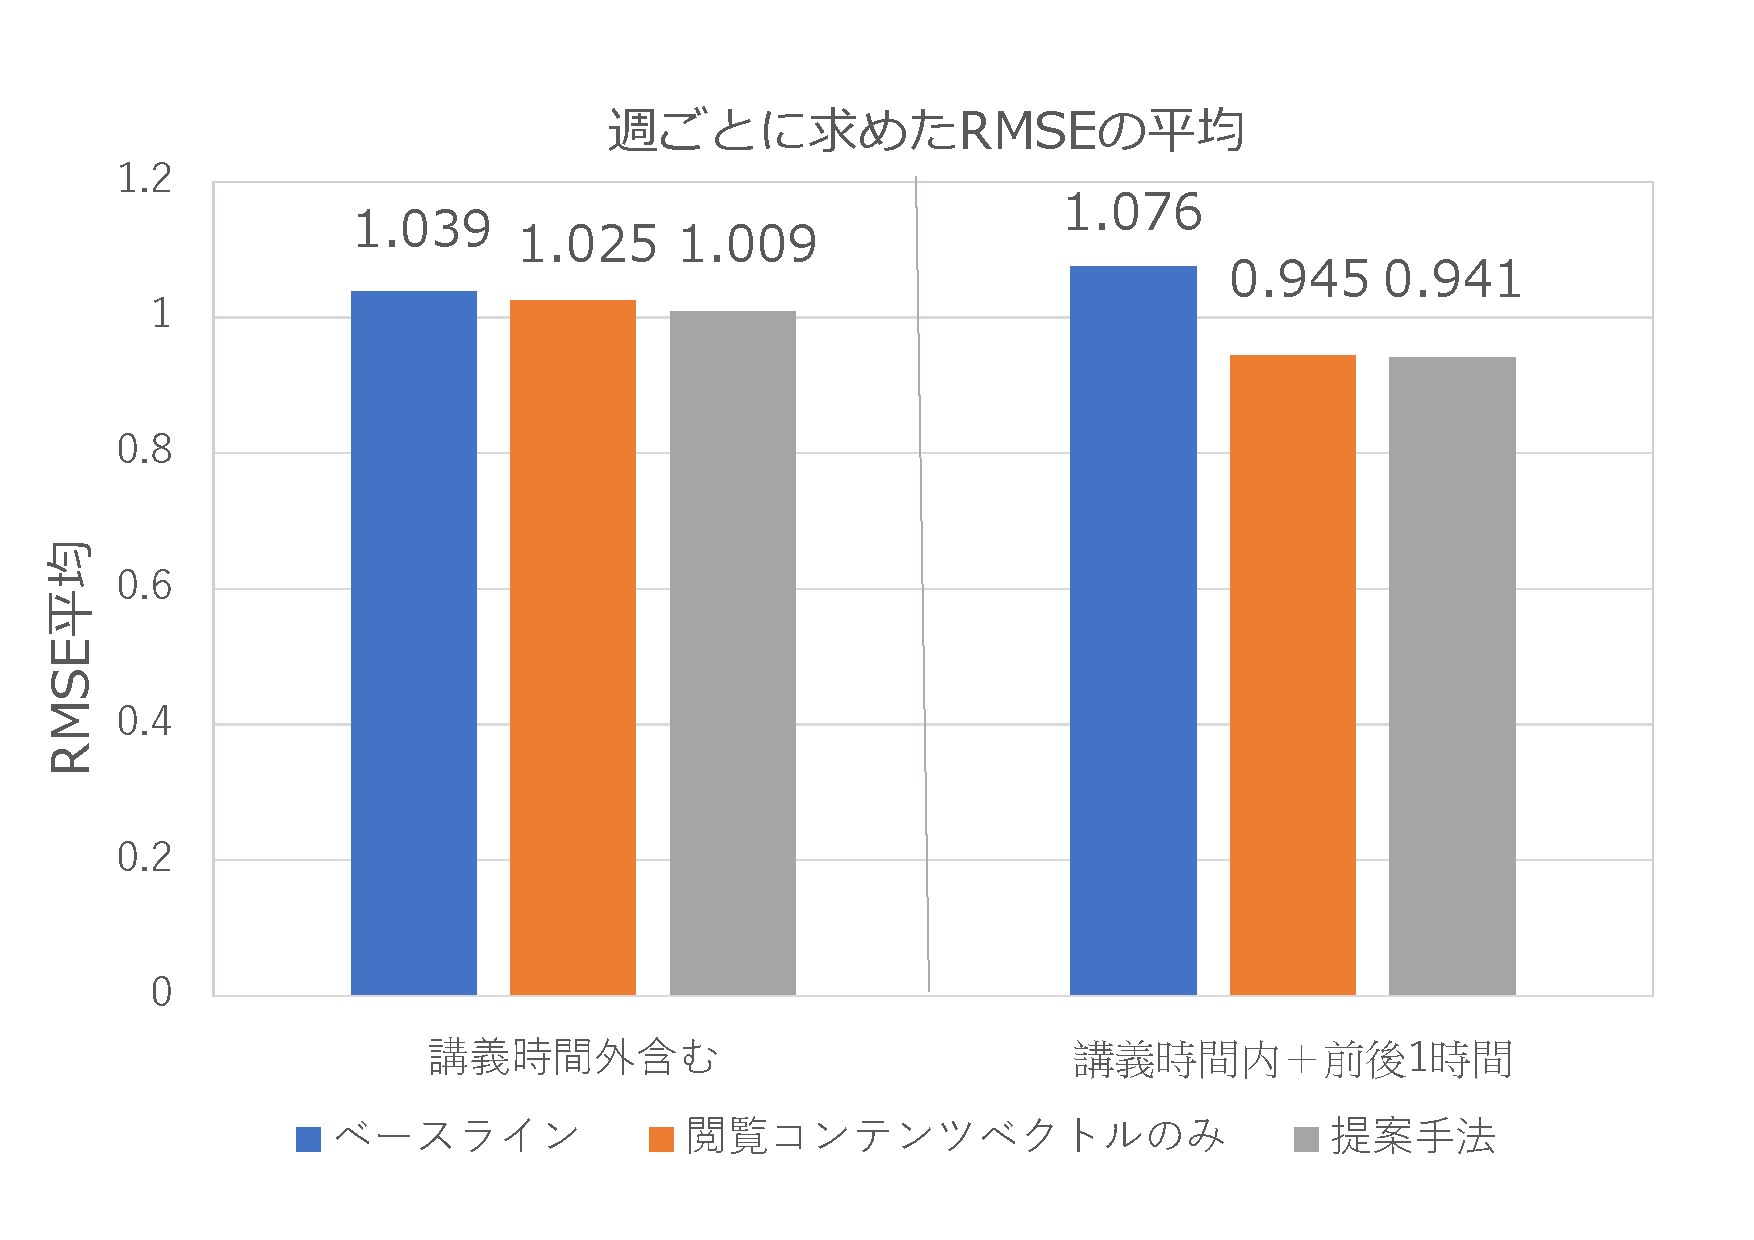
\includegraphics[scale = 0.35]{RMSE.pdf}
  % 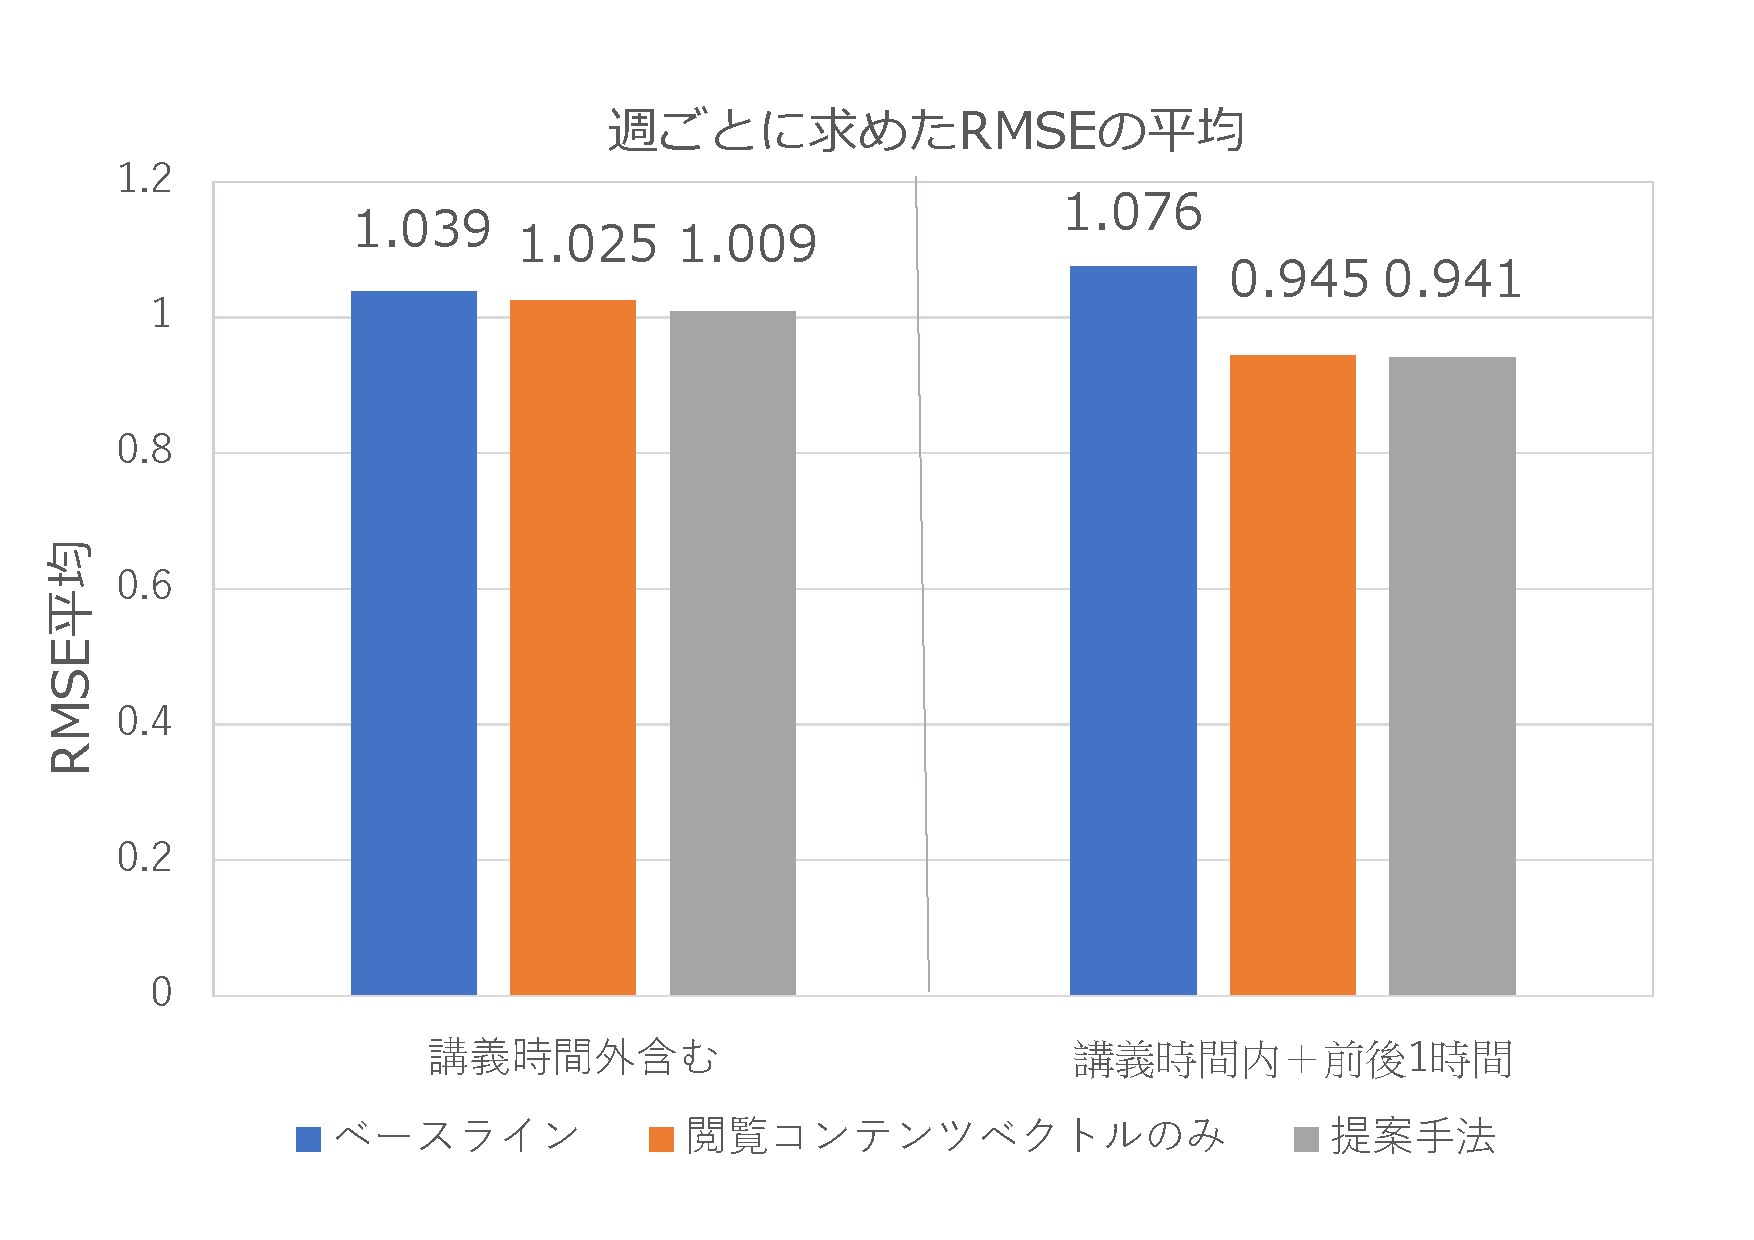
\includegraphics[width=\linewidth]{RMSE.pdf}
  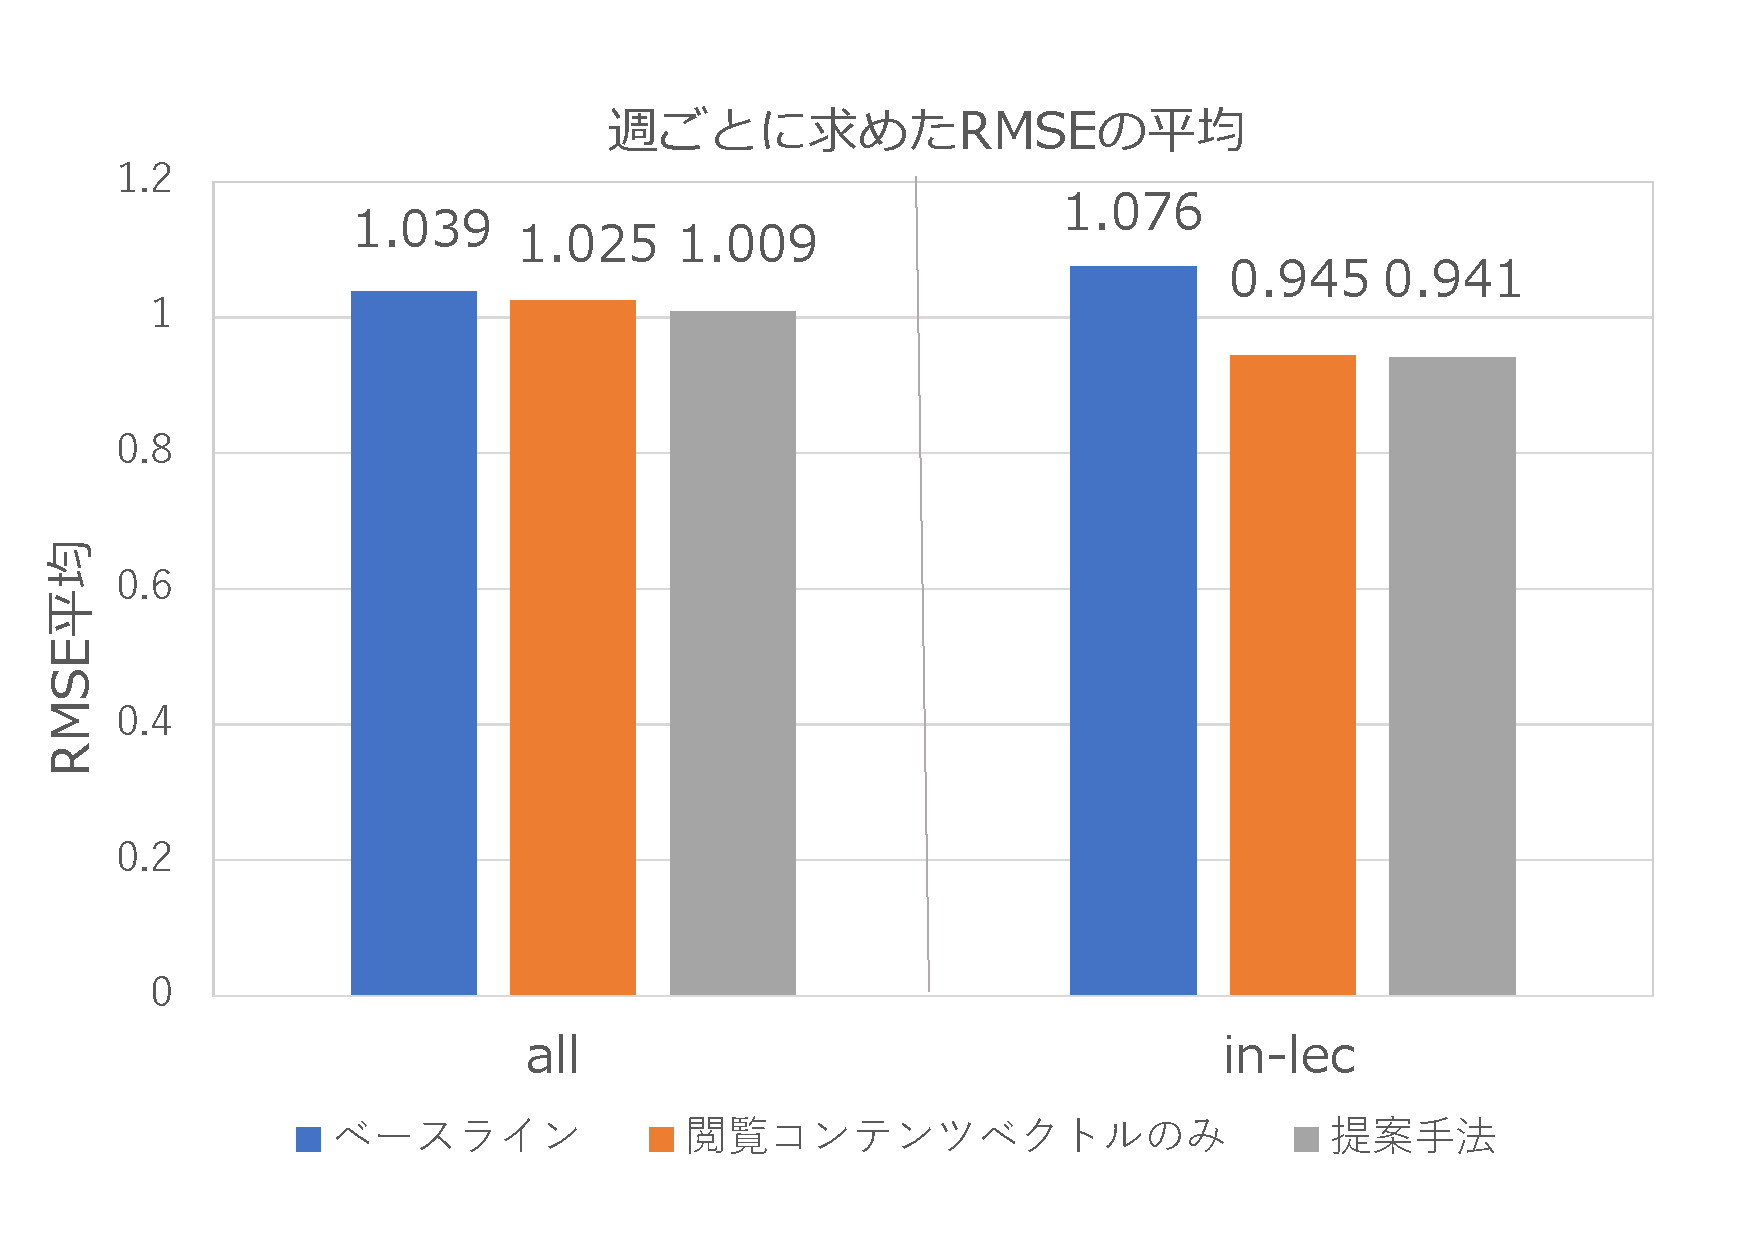
\includegraphics[width=\linewidth]{RMSE_.pdf}
  % \vspace{-5mm}
  \caption{小テストごとに求めたRMSEの平均}
  \label{fig:rmse}
  \vspace{-5mm}
\end{figure}



%\begin{table}[h]
% \begin{table}[h]
%   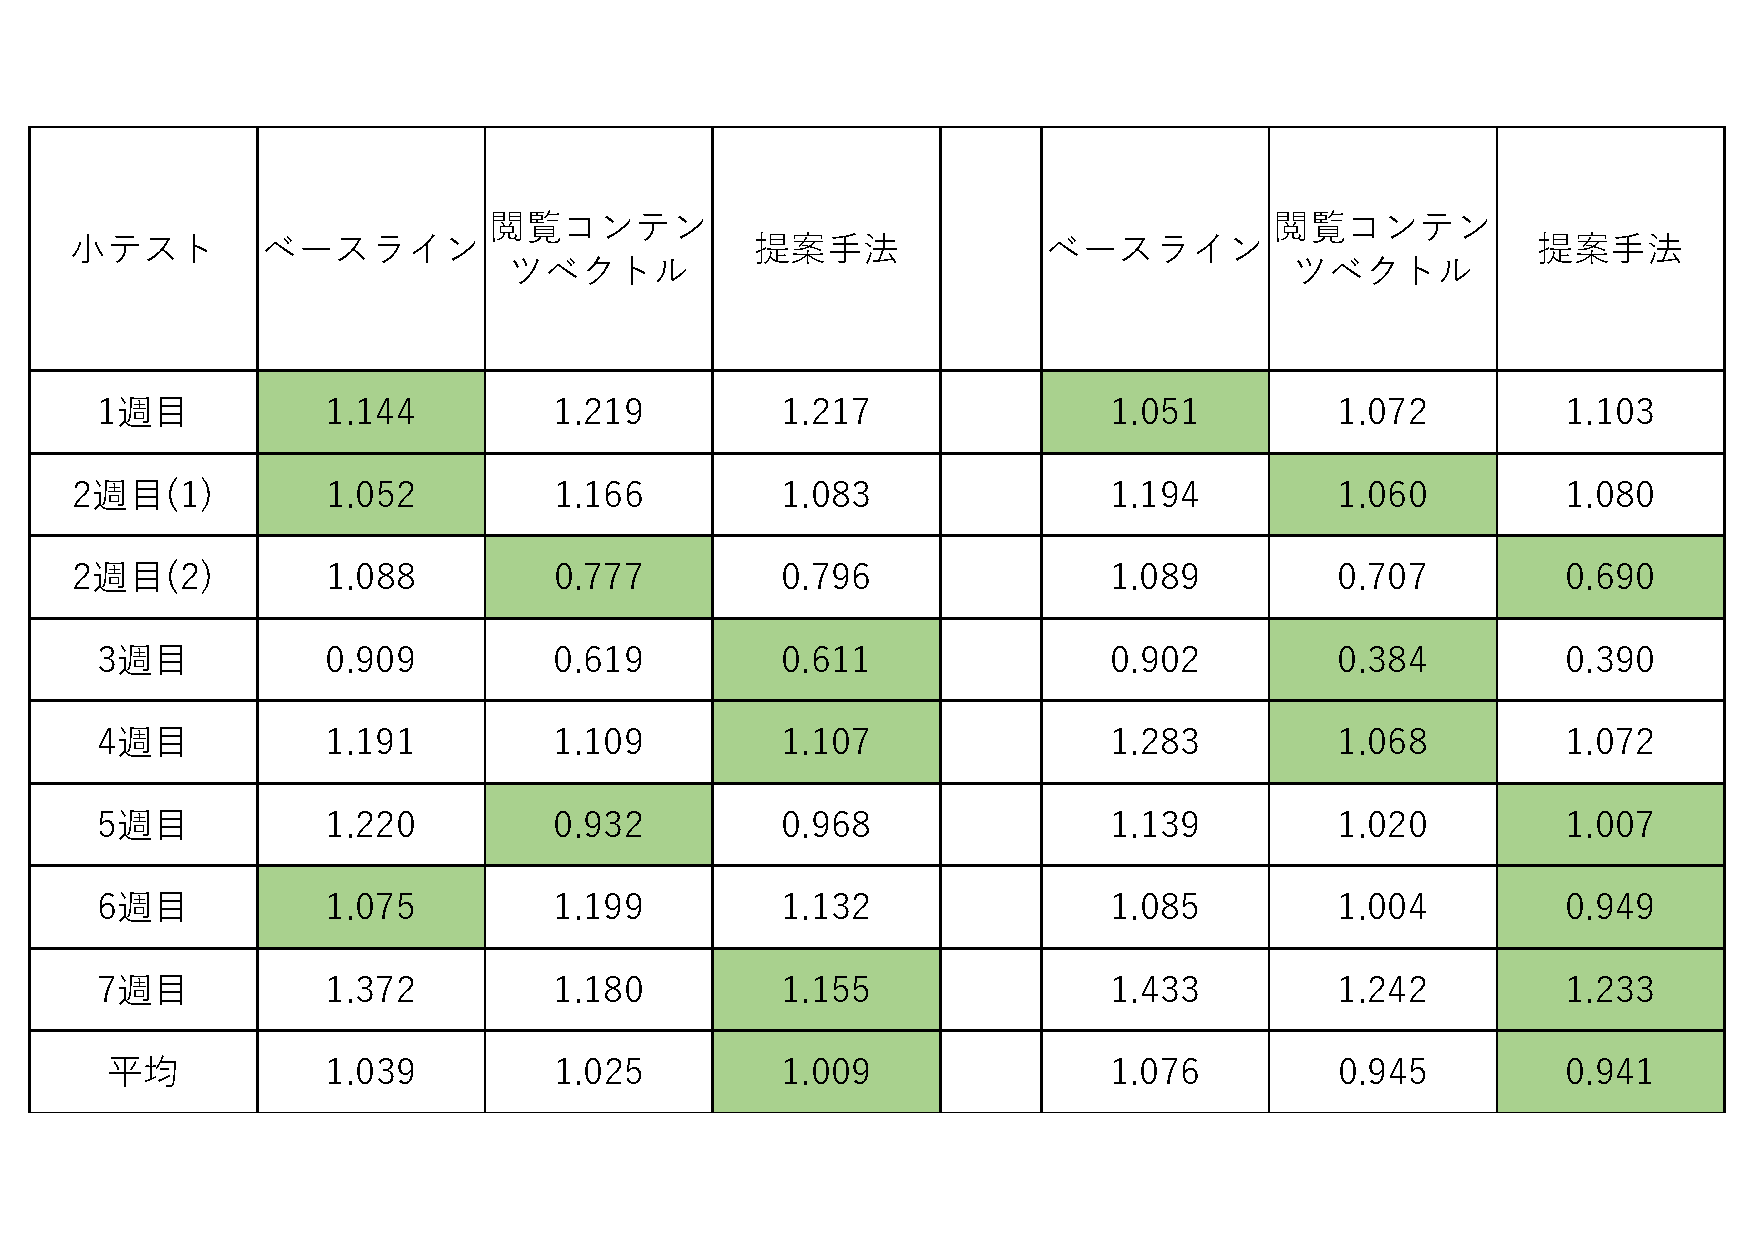
\includegraphics[width=0.9\linewidth]{RMSEhyov3_.pdf}
%   \caption{小テストごとの平均RMSE(左2列: 講義時間外含む.右2列: 講義時間内および前後1時間)}
%   % \vspace{-5mm}
%   \label{tab:rmse_each}
%   \centering
%   %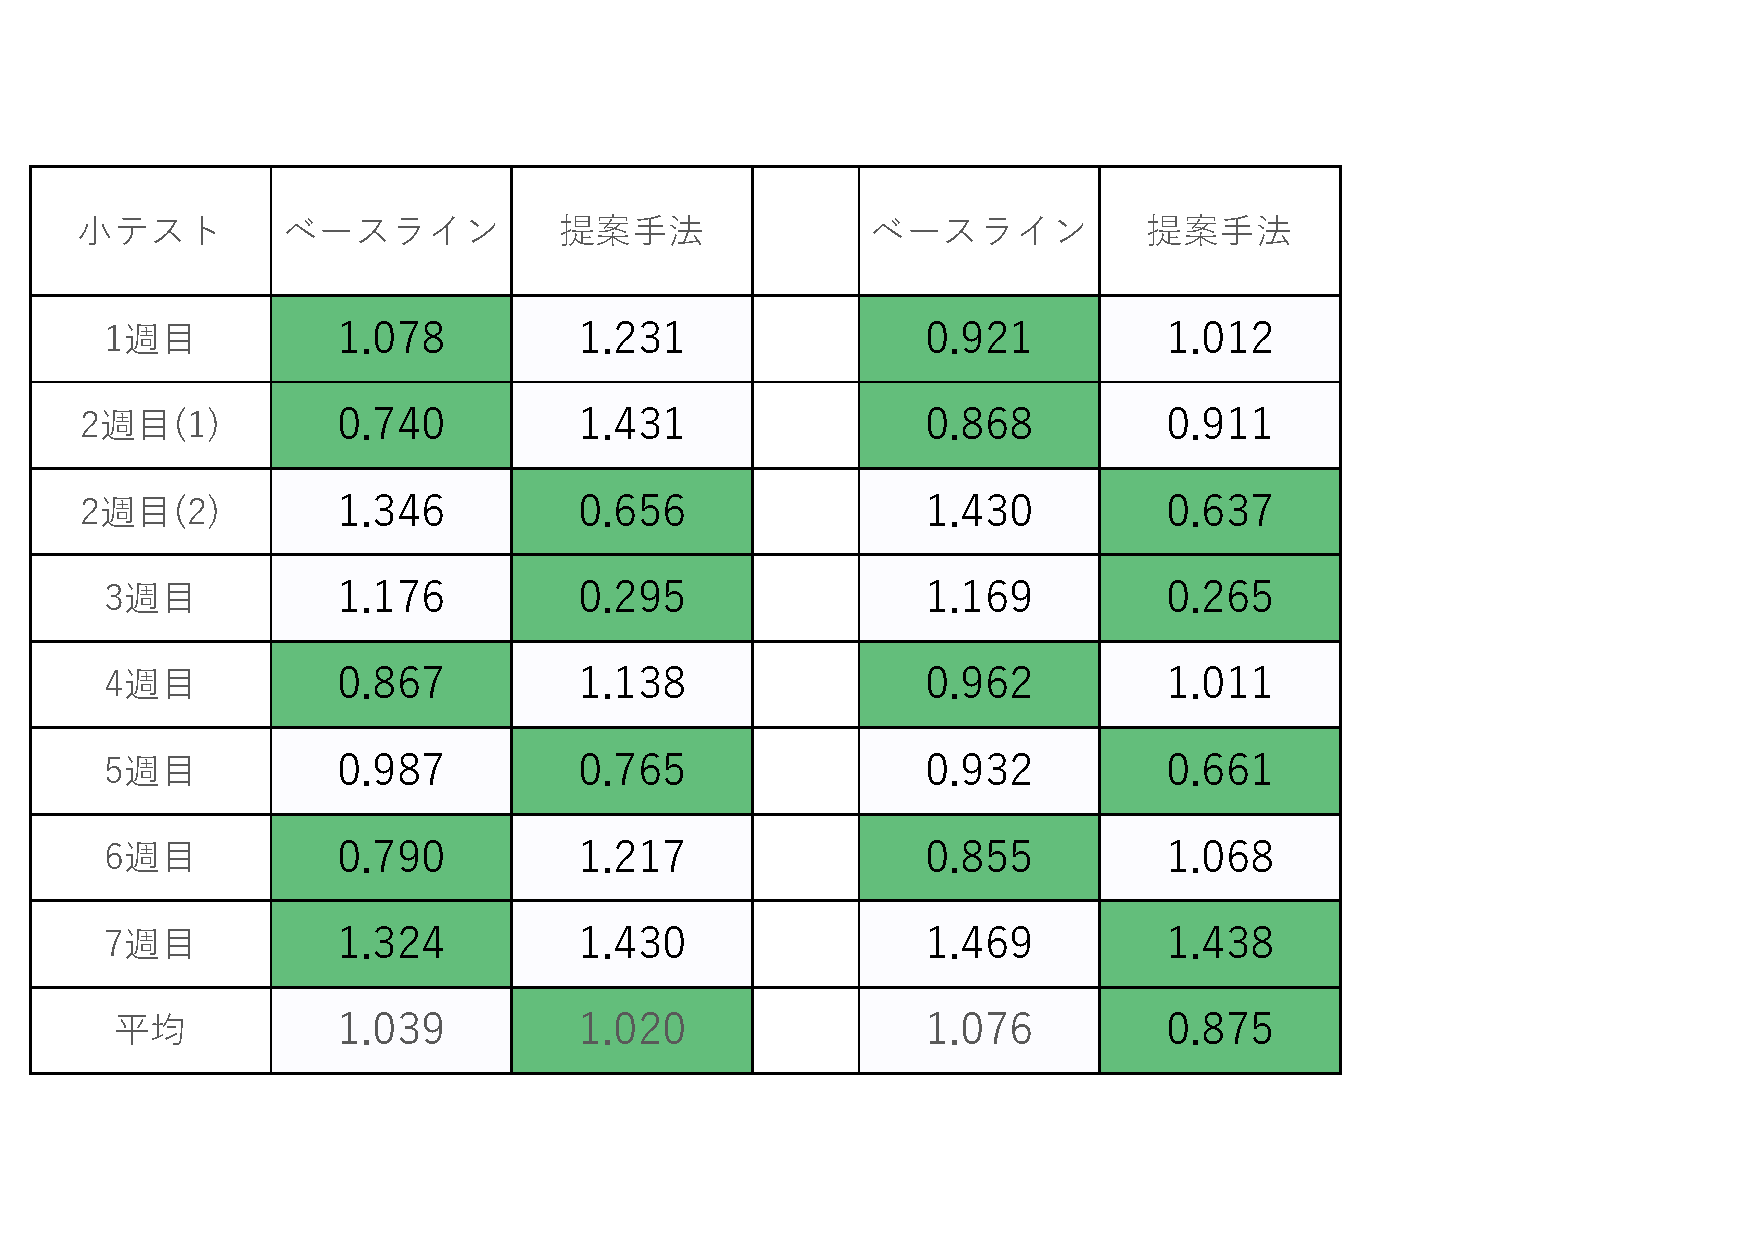
\includegraphics[scale = 0.3]{RMSEhyov3.pdf}
% \end{table}


\subsection{課題}
% 課題?考察?まとめ?
結果から,学生の行動を講義時間内(前後1時間含む)に絞ることはスコア予測の精度向上に繋がる.また,ベースラインと比べて提案手法ではRMSEの値が下がっていることよりコンテンツ情報を含めることはスコア予測の精度向上に繋がり,学習行動の中では各ページの閲覧時間がより重要であると言える.
本研究では実験していないが,行動の重要度に加え,ページの重要度を変えることでより高い精度を期待できる.
%のではないだろうか.



\vspace{2mm}
\noindent{\bf 謝辞} \quad
本研究の一部は科研費JP19H04226の補助を受けて行った.

% https://www.jsps.go.jp/j-grantsinaid/16_rule/rule.html#shaji


{
\footnotesize
% \bibliographystyle{jplain}  % LastNameのアルファベット順
\bibliographystyle{junsrt}  % 引用順
\bibliography{ipsjkogishi}  % sample.bib の場合(bibファイル名に合わせて変更すること)
%% bibtex を使わない場合は上の2行をコメントアウトして以下に列挙

% ちょっと微妙journalとかになにかけばいいかにわからないです.
% 論文あった場所bibにおいてます.


% \begin{thebibliography}{10}
% \bibitem{Rodrigue:IUI2015}
% M. Rodrigue, J. Son, B. Giesbrecht, M. Turk, T. H\"{o}llerer.
% \newblock Spatio-Temporal Detection of Divided Attention in Reading Applications Using EEG and Eye Tracking.
%   \newblock In {\em IUI}, pages 121--125. 2015.
% \end{thebibliography}
}


\end{document}
